\documentclass[a4paper,12pt]{article}

\usepackage[russian]{babel} % Язык документа

% Подключаем fontspec для управления шрифтами
\usepackage[T1]{fontenc}
\usepackage[utf8]{inputenc}


\usepackage{geometry}
\geometry{left=30mm, right=10mm, top=20mm, bottom=20mm}

\usepackage{setspace}
\onehalfspacing
\setlength{\parindent}{15mm}

\usepackage{graphicx}
\usepackage{caption}
\usepackage{booktabs}
\usepackage{amsmath}
\usepackage{tocloft}
\usepackage{titlesec}
\usepackage{float}
\usepackage{hyperref}
\usepackage{listings}
\usepackage{xcolor}

\lstset{
	language=Python,
	basicstyle=\ttfamily\small,
	keywordstyle=\color{blue}\bfseries,
	stringstyle=\color{red},
	commentstyle=\color{green!50!black},
	numbers=left,
	numberstyle=\tiny,
	stepnumber=1,
	numbersep=5pt,
	showspaces=false,
	showstringspaces=false,
	frame=none,
	breaklines=true,
	breakatwhitespace=true,
	tabsize=2,
	columns=fullflexible,
	mathescape=false,
}

\titleformat{\section}{\normalfont\bfseries}{\thesection}{1em}{}
\titleformat{\subsection}{\normalfont\bfseries}{\thesubsection}{1em}{}

% Форматирование титульной страницы
\begin{document}

\begin{titlepage}
	\vspace*{1cm}
	{\small
		\begin{center}
			МИНИСТЕРСТВО НАУКИ И ВЫСШЕГО ОБРАЗОВАНИЯ РОССИЙСКОЙ ФЕДЕРАЦИИ\\
			ФЕДЕРАЛЬНОЕ ГОСУДАРСТВЕННОЕ АВТОНОМНОЕ ОБРАЗОВАТЕЛЬНОЕ УЧРЕЖДЕНИЕ ВЫСШЕГО ОБРАЗОВАНИЯ\\
			\textbf{НАЦИОНАЛЬНЫЙ ИССЛЕДОВАТЕЛЬСКИЙ ТОМСКИЙ ПОЛИТЕХНИЧЕСКИЙ УНИВЕРСИТЕТ}
		\end{center}
	}
	\vspace{0.5cm}
	\begin{center}
		Инженерная школа информационных технологий и робототехники\\
		Отделение информационных технологий\\
		Направление: 09.04.01 Искусственный интеллект и машинное обучение
	\end{center}
	\vspace{1cm}
	\begin{center}
		\textbf{ОТЧЁТ ПО ПРАКТИЧЕСКОЙ РАБОТЕ}
	\end{center}
	\begin{center}
		по дисциплине: Нейроэволюционные вычисления
	\end{center}
	\vspace{0.5cm}
	% Добавление "Вариант 21" по центру
	\begin{center}
		\textbf{Вариант 14}
	\end{center}
	\begin{center}
		на тему: Реализация алгоритма нейроэволюции H-ESP для непрерывного контроля среды Lunar Lander
	\end{center}
	\vspace{1cm}
	
	% Двухколоночное расположение
	\begin{tabular}{p{0.3\textwidth} p{0.35\textwidth} p{0.3\textwidth}}
		\textbf{Выполнил:} & студент гр. 8ВМ42 \newline Мабах А.С. & 09.06.2025 \\
		& & \\
		\textbf{Проверил:} & к.т.н., Доцент ОИТ ИШИТР \newline Григорьев Д.С. & 09.06.2025
	\end{tabular}
	\vfill
	\begin{center}
		Томск – 2025
	\end{center}
\end{titlepage}


% Оглавление
\tableofcontents
\setcounter{page}{2}
\newpage

% Настройка форматирования разделов и интервалов
\titleformat{\section}{\normalfont\bfseries}{\thesection}{1em}{}
\titleformat{\subsection}{\normalfont\bfseries}{\thesubsection}{1em}{}
\setlength{\parindent}{15mm}
\onehalfspacing

% Раздел 1: Введение
\section{Введение}

\textbf{Цель работы} — реализовать полный цикл нейроэволюционного обучения с помощью алгоритма H-ESP для задачи управления агентом в среде \texttt{LunarLander-v3}, соблюдая следующие требования:
\begin{itemize}
	\item Разработка модульного и воспроизводимого кода без использования сторонних реализаций H-ESP;
	\item Детальная визуализация структуры сети и динамики обучения на каждом этапе;
	\item Обоснование и анализ используемых целевых метрик, обеспечивающих объективную оценку успешности обучения.
\end{itemize}

\newpage
% Раздел 2: Описание алгоритма
\section{Описание используемого алгоритма}

\subsection{Принципы работы H-ESP (Hierarchical Enforced SubPopulations)}
Алгоритм H-ESP (Hierarchical Enforced SubPopulations), предложенный Фаустино Гомесом как вариант развития ESP.Нововведением является использование эволюции уровня сетей (L1), а не только нейронов (L2).


\subsection{Структура сети}
В работе используется рекуррентная нейронная сеть (RNN), которая обрабатывает последовательные данные с сохранением внутреннего состояния подходящая под алгоритм H-ESP:
\begin{itemize}
	\item \textbf{Входной слой:} Полносвязный слой (Linear), преобразующий входные данные в скрытое пространство.
	\item \textbf{Рекуррентный слой:} Обрабатывает предыдущее скрытое состояние.
	\item \textbf{Выходной слой:} Преобразует скрытое состояние в выходные данны
\end{itemize}


\subsection{Этапы алгоритма H-ESP}
Алгоритм H-ESP состоит из следующих этапов:
\begin{enumerate}
	\item \textbf{Инициализация}
	\begin{itemize}
		\item Задаётся число скрытых нейронов $h$.
		\item Формируется $N$ случайных сетей с $h$ скрытыми нейронами.
	\end{itemize}
	\item \textbf{Оценка приспособленности (Evaluation)}
	\begin{itemize}
		\item Уровень нейронов. Если полученная при оценивании сеть лучше, чем худшая сеть из L2, то она добавляется в L2.
		\item Уровень нейронных сетей. Формируется NN случайных сетей с hh скрытыми нейронами.
    \begin{itemize}
        \itemОпределяется приспособленность еще не оцененных сетей.
        \itemЕсли приспособленность сети лучше, чем приспособленность лучшей ИНС (искусственной нейронной сети) из L1, то нейроны из этой сети добавляются в подпопуляции.
	\end{itemize}
    \end{itemize}
	\item \textbf{Проверка вырождения популяции}
	\begin{itemize}
		\item Если лучшая приспособленность не улучшается на протяжении $b$ поколений, применяется взрывная мутация (``burst mutation''): подпопуляции перегенерируются вблизи своих лучших особей с помощью распределения Коши.
		\item Если и после двух взрывных мутаций улучшения нет, применяется адаптация структуры сети  --- изменение количества подпопуляций/нейронов.
	\end{itemize}
	\item \textbf{Скрещивание (Crossover) и отбор (Selection)}
    \begin{itemize}
    \item Уровень нейронов
	\begin{itemize}
		\item Для каждой подпопуляции рассчитывается средний фитнес каждой особи (суммарный фитнес делится на число испытаний).
		\item Особей сортируют по убыванию приспособленности; лишние особи (выходящие за пределы размера популяции) удаляются.
		\item Лучшие особи (обычно 1/4) скрещиваются между собой (одноточечный кроссовер), потомки добавляются в конец подпопуляции.
		\item Для нижней половины популяции применяется мутация с распределением Коши.
	\end{itemize}
    \item Уровень нейронных сетей. Каждая ИНС скрещивается с более приспособленной с использованием h-точечного кроссинговера («понейронно»). Потомки мутируют.
    \end{itemize}
	\item \textbf{Повторение}
	\begin{itemize}
		\item Шаги 2--4 повторяются до выполнения критерия остановки (например, достижение целевого качества или максимального числа эпох).
	\end{itemize}
	
    
    
\end{enumerate}


\newpage
\section{Этапы имплементации}

Реализация алгоритма H-ESP для задачи управления в среде \texttt{LunarLanders-v3} была выполнена на языке Python с использованием только стандартных научных библиотек. (\texttt{numpy}, \texttt{gymnasium}) и полностью авторской логики без сторонних реализаций нейроэволюции. Оригинальный алгоритм был несколько переработан для оптимизации под конкретную задачу.

\subsection{Модульная структура кода}

Код организован модульно, что облегчает повторное использование и дальнейшее расширение:
\begin{itemize}
	\item \textbf{Модуль \texttt{Model}} — реализует основные эволюционные операции и логику подпопуляций.
	\item \textbf{Модуль \texttt{Network}} — отвечает за архитектуру сети.
	\item \textbf{Вспомогательные модули} — визуализация, сохранение/загрузка весов, утилиты командной строки.
	\item \textbf{Главный исполняемый файл} — обеспечивает запуск обучения, тестирования и визуализации через аргументы командной строки.
\end{itemize}

\subsection{Основные этапы реализации}

\paragraph{Инициализация}~\\ 

В оригинальном алгоритме инициализация состоит в создании случайных сетей и их добавлении в подпопуляции L2, если они оказываются более приспособленными. Также в процессе инициализации определяются признаки для каждой сети. В данной реализации же инициализация происходит через создание случайных сетей для уровня L1, каждая из которых оценивается в среде и добавляется в популяцию. Здесь создается только один уровень, в отличие от оригинала, где можно увидеть более сложную структуру с уровнями L1 и L2, с добавлением нейронов в зависимости от их приспособленности.~\\
Реализация подпопуляции в коде: 
    \begin{itemize}
	
	\begin{lstlisting}
		self.L1 = []
        
        for _ in range(L1_size):
            net = ReccurentNetwork(self.input_dim, self.output_dim, hidden_units)
            self.evaluate_network(net)
            self.L1.append(net)
	\end{lstlisting}
    \end{itemize}
  
\paragraph{Оценка приспособленности}~\\ 

В оригинальном алгоритме оценка приспособленности заключается в расчетах на основе симуляции сети и различных пробежек по поколениям. Каждый нейрон оценивается на основе своих попыток при определении приспособленности, что является более теоретическим процессом. В коде же оценка приспособленности происходит через вычисление общего вознаграждения на нескольких эпизодах в игре. Каждая сеть, проходя через среду, получает свою оценку на основе общего вознаграждения, что делает этот процесс более специфичным и привязанным к задаче, в отличие от теоретического подхода, который используется в оригинальном алгоритме.~\\ 
Каждая сеть проходит оценку через функцию evaluate\_network, где вычисляется её приспособленность на основе суммы вознаграждений за несколько эпизодов.~\\ 
Реализация оценки приспособленности в коде:
	\begin{itemize}
        
        \begin{lstlisting}
        def evaluate_network(self, network, episodes=5, render=False):
            total_reward = 0
            for _ in range(episodes):
                state, _ = self.env.reset()
                network.reset_states()
                done = False
                while not done:
                    action = np.argmax(network.predict(state))
                    state, reward, terminated, truncated, _ = self.env.step(action)
                    done = terminated or truncated
                    total_reward += reward
        
            fitness = total_reward / episodes
            network.fitness = fitness

        \end{lstlisting}
	\end{itemize}
	


\paragraph{Рекомбинация подпопуляций}~\\ 

В оригинальном алгоритме рекомбинация происходит внутри подпопуляций нейронов с использованием их признаков и приспособленности для создания новых сетей. В коде этот процесс происходит через выбор двух лучших сетей из L1 для скрещивания, с последующим использованием кроссинговера и мутации. Кроссинговер, как и в оригинале, происходит между сетями, но в коде это делает случайный выбор двух сетей, что влияет на разнообразие в процессе. В оригинале акцент больше сделан на подпопуляции, где каждая группа имеет свои особенности, а в коде это более примитивный выбор между лучшими особями.
Рекомбинация происходит через выбор двух лучших сетей из L1, которые затем проходят процесс кроссинговера и мутации.~\\ 
Реализация рекомбинации:
\begin{itemize}
        
        \begin{lstlisting}
        def recombine(self):
            new_pop = []
            sorted_L1 = sorted(self.L1, key=lambda x: x.fitness, reverse=True)
            topk = sorted_L1[:max(2, len(sorted_L1)//3)]
            
            while len(new_pop) < self.population_size:
                p1 = random.choice(topk)
                p2 = random.choice(topk)
                if p2 is p1:
                    continue
                child = p1.crossover(p2)
                
                child.mutate(L2_pool=self.L2)  
                
                new_pop.append(child)
            return new_pop
        \end{lstlisting}
	\end{itemize}

\paragraph{Обновление уровня сетей}~\\

В оригинальном алгоритме обновление уровня сетей включает добавление новых сетей в L2, а также их оценку и возможную замену худших. Это происходит на основе приспособленности, когда нейроны из сетей с высокой приспособленностью добавляются в L2, что влияет на будущие поколения. В коде же обновление происходит через добавление нейронов в L2 с учетом их приспособленности и замены худших нейронов, если появляется новый более подходящий нейрон. Здесь больше внимания уделяется замене нейронов в списке L2, чем в оригинальном алгоритме, где добавление новых сетей в подпопуляции более структурировано.~\\
Обновление уровня сетей происходит через добавление лучших нейронов в L2, если их приспособленность выше определённого уровня, и через замену худших нейронов.~\\
Реализация обновления сетей:
\begin{itemize}
	\item[] Реализация операций:
	\begin{lstlisting}
		for i in range(len(self.networks)):
        if self.network_fitness[i] == -float('inf'):
            self.network_fitness[i] = self.evaluate_network(self.networks[i], env)

        best_net_idx = np.argmax(self.network_fitness)
        best_net = self.networks[best_net_idx]
        for i in range(self.hidden_size):
            neuron_weights = torch.cat([best_net.fc1.weight[i], best_net.fc1.bias[i], best_net.recurrent.weight[i]])
            worst_idx = np.argmin(self.subpop_fitness[i])
            self.subpopulations[i][worst_idx] = neuron_weights
	\end{lstlisting}
\end{itemize}




\paragraph{Рекомбинация сетей}~\\

В оригинальном алгоритме рекомбинация сетей основана на слиянии сетей с лучшими признаками и их приспособленностью. Это может подразумевать более общий подход к слиянию сетей. В коде же процесс рекомбинации реализован через кроссинговер между двумя сетями, с выбором нейронов, принадлежащих к одному из родителей. Этот процесс более конкретен, так как каждый нейрон из скрытых слоев или выходных нейронов копируется случайным образом из одной из двух сетей. Это делает процесс более направленным на случайность и изменчивость в составе сетей, что отличается от абстрактного описания в оригинальном алгоритме.~\\
В коде рекомбинация сетей осуществляется через кроссинговер между двумя сетями с использованием случайного выбора нейронов из разных сетей.~\\
Реализаци рекомбинации сетей в коде:
    \begin{itemize}
	\begin{lstlisting}
		def crossover(self, other):
            child = ReccurentNetwork(self.input_dim, self.output_dim, self.hidden_units)
            for i in range(self.hidden_units):
                parent = self.hidden_neurons[i] if random.random() < 0.5 else other.hidden_neurons[i]
                child.hidden_neurons[i] = parent.clone()
            for i in range(self.output_dim):
                parent = self.output_neurons[i] if random.random() < 0.5 else other.output_neurons[i]
                child.output_neurons[i] = parent.clone()
            return child

	\end{lstlisting}
\end{itemize}



\begin{itemize}
	\item[] Логика адаптации:
	\begin{lstlisting}
		for i in range(self.num_subpops):
        best_idx = np.argmax(self.subpop_fitness[i])
        best_neuron = self.subpopulations[i][best_idx]
        self.subpopulations[i] = [self.cauchy_mutation(best_neuron, self.mutation_scale) 
                                for _ in range(self.subpop_size)]
	\end{lstlisting}
\end{itemize}





\newpage
\section{Целевые метрики}

\subsection{Формальное определение метрики}
Основной целевой метрикой является \textbf{среднее суммарное вознаграждение за эпизод} (average episodic reward), вычисляемое как:

\[
R_{\text{avg}} = \frac{1}{N} \sum_{i=1}^{N} R_i
\]

где:
\begin{itemize}
	\item $N$ — количество эпизодов оценки
	\item $R_i$ — суммарное вознаграждение за $i$-й эпизод
\end{itemize}

\subsection{Расчёт вознаграждения в LunarLanderContinuous-v3}
В среде \texttt{LunarLander-v3} вознаграждение формируется по сложной формуле, учитывающей физические параметры посадки:

\[
R = R_{\text{position}} + R_{\text{velocity}} + R_{\text{angle}} + R_{\text{contact}} + R_{\text{landing}} + R_{\text{fuel}} + R_{\text{time}}
\]

Компоненты вознаграждения:
\begin{enumerate}
	\item \textbf{Позиция} ($R_{\text{position}}$): 
	\[
	-100 \sqrt{(x - x_{\text{target}})^2 + (y - y_{\text{target}})^2}
	\]
	Штраф за удаление от целевой зоны посадки
	
	\item \textbf{Скорость} ($R_{\text{velocity}}$):
	\[
	-100 \left( |v_x| + |v_y| \right)
	\]
	Штраф за высокую горизонтальную ($v_x$) и вертикальную ($v_y$) скорость
	
	\item \textbf{Угол наклона} ($R_{\text{angle}}$):
	\[
	-100 |\theta|
	\]
	Штраф за отклонение от вертикального положения ($\theta$ — угол в радианах)
	
	\item \textbf{Контакт с поверхностью} ($R_{\text{contact}}$):
	\[
	+10 \cdot (\text{leg1\_contact} + \text{leg2\_contact})
	\]
	Награда за касание посадочными опорами
	
	\item \textbf{Успешная посадка} ($R_{\text{landing}}$):
	\[
	\begin{cases} 
		+200 & \text{если } v_y > -1 \text{ м/с и } |\theta| < 0.2 \text{ рад} \\
		-100 & \text{в противном случае}
	\end{cases}
	\]
	
	\item \textbf{Расход топлива} ($R_{\text{fuel}}$):
	\[
	-0.3 \cdot (\text{main\_engine} + 0.03 \cdot \text{side\_engine})
	\]
	Штраф за использование основного и боковых двигателей
	
	\item \textbf{Временной штраф} ($R_{\text{time}}$):
	\[
	-0.3 \cdot t
	\]
	Штраф за каждый шаг симуляции ($t$)
\end{enumerate}

\subsection{Реализация в системе обучения}
В системе обучения метрика рассчитывается следующим образом:

\begin{lstlisting}[language=Python]
    best = max(n.fitness for n in self.L1)
    avg = np.mean([n.fitness for n in self.L1])

    fitness = total_reward / episodes
    network.fitness = fitness
\end{lstlisting}

\subsection{Интерпретация метрики}
\begin{itemize}
	\item \textbf{Успешная посадка}: $R_{\text{avg}} \geq 200$ 
	\item \textbf{Приемлемый результат}: $50 \leq R_{\text{avg}} < 200$
	\item \textbf{Неудачная посадка}: $R_{\text{avg}} < 0$
	\item \textbf{Рекорд среды}: $R_{\text{avg}} \approx 300$ (оптимальная посадка)
\end{itemize}


\newpage
\section{Визуализация}

Важной частью анализа эволюционного обучения является наглядная визуализация развития структуры нейронной сети и динамики ключевых метрик. В ходе экспериментов автоматически сохранялись скриншоты архитектуры сети на различных этапах (через фиксированный интервал эпох), а также строились графики изменения целевых показателей.

\subsection{Визуализация структуры нейронной сети}

На рисунках ниже представлены архитектуры реккурентной нейронной сети с одним скрытым слоем, эволюционирующей с помощью алгоритма H-ESP для задачи управления посадкой в среде \texttt{LunarLander-v3}. Входными данными для сети служат восемь параметров состояния среды (позиция, скорость, угол, контакт с поверхностью и др.), скрытый слой состоит из 12 нейронов, выходной слой --- из 4 нейрона, отвечающих за одно из возможных действий.

Каждая визуализация строится по ``лучшей'' сети --- она собирается из лучших особей каждой подпопуляции на данной эпохе.


На каждом изображении (рис. \ref{fig:network_legend}):
\begin{itemize}
	\item \textbf{Цвет и толщина связей} отражают знак и величину весового коэффициента:
	\begin{itemize}
		\item \textcolor{green}{Зеленые линии} --- положительные веса (активирующие связи)
		\item \textcolor{red}{Красные линии} --- отрицательные веса (ингибирующие связи)
        \item Пунктрирные линии - реккурентная связь
		\item Толщина линии пропорциональна абсолютной величине веса $|w|$
	\end{itemize}
	\item \textbf{Нормализация}: Для устранения влияния выбросов толщина и насыщенность масштабируются по 95-му перцентилю модулей весов
	\item \textbf{Узлы сети}:
	\begin{itemize}
		\item \textcolor{gray}{Серые} --- входные нейроны
		\item \textcolor{blue}{Синие} --- реккурентный слой
		\item \textcolor{orange}{Оранжевый} --- выходные нейроны
	\end{itemize}


Пример визуализации структуры сети:


\begin{figure}[H]
	\centering
	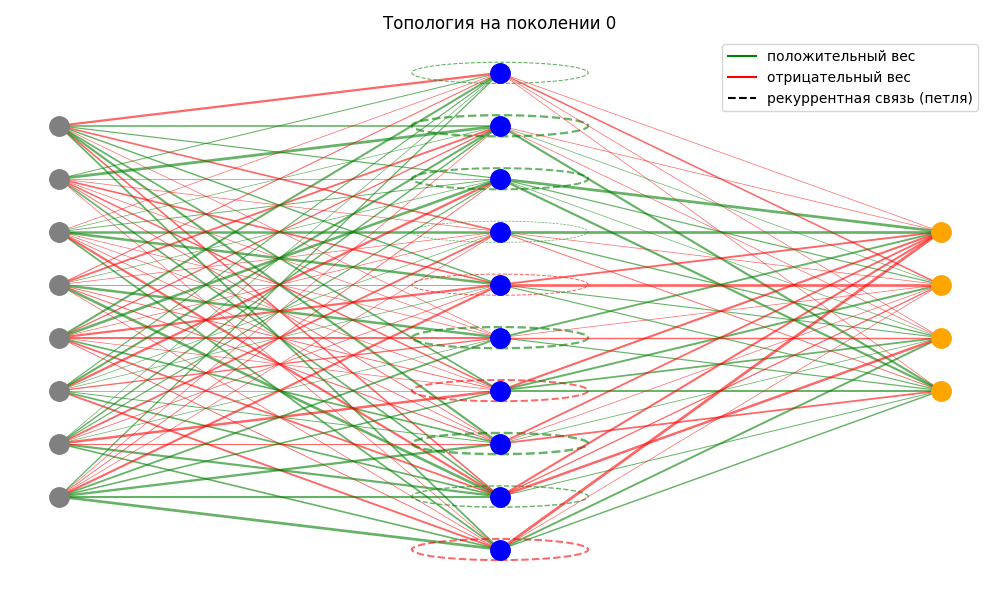
\includegraphics[width=0.95\textwidth]{topology_gen_0.png}
	\caption{Визуализизация структуры сети после инициализации}
	\label{fig:test_results}
\end{figure}


\begin{figure}[H]
	\centering
	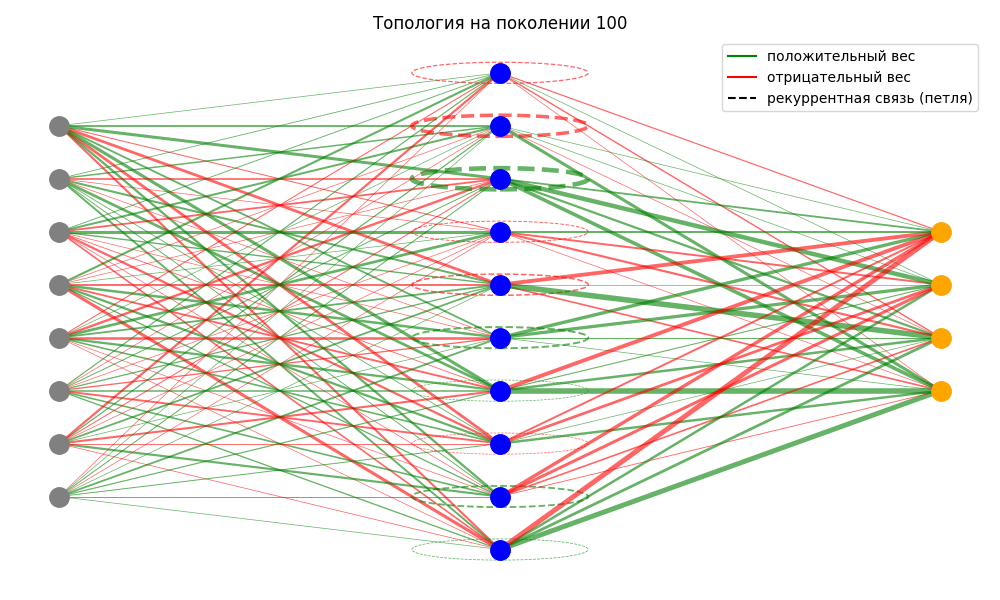
\includegraphics[width=0.95\textwidth]{topology_gen_100.png}
	\caption{Визуализизация структуры сети на 100 поколении}
	\label{fig:test_results}
\end{figure}

\begin{figure}[H]
	\centering
	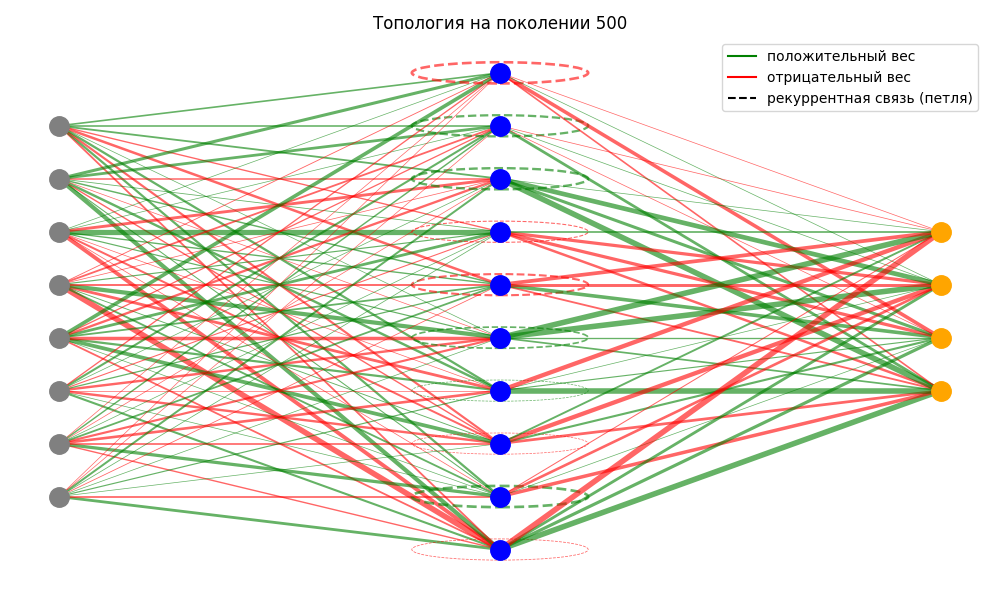
\includegraphics[width=0.95\textwidth]{topology_gen_500.png}
	\caption{Визуализизация структуры сетина 500 поколении}
	\label{fig:test_results}
\end{figure}

\begin{figure}[H]
	\centering
	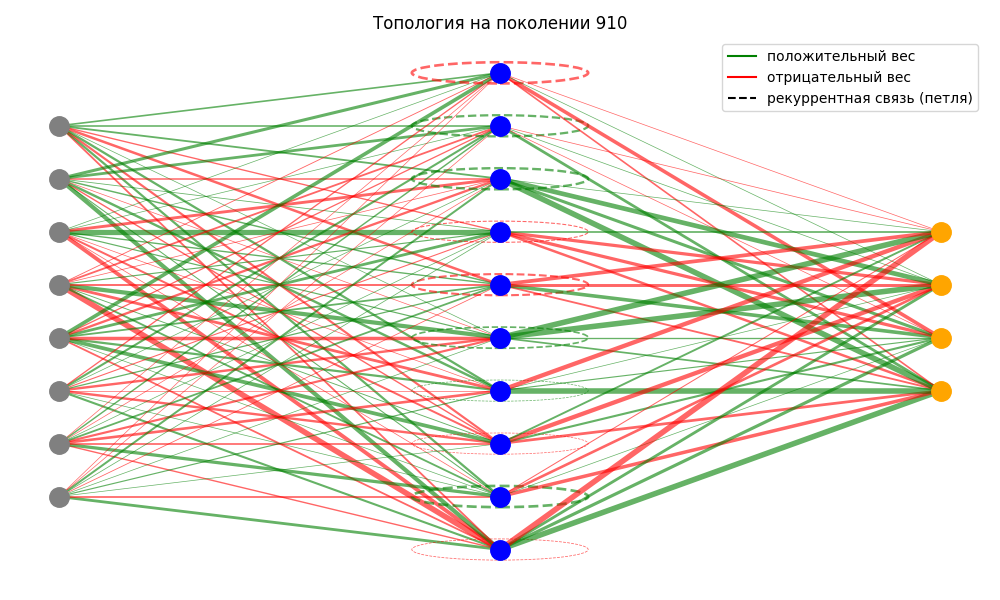
\includegraphics[width=0.95\textwidth]{topology_gen_910.png}
	\caption{Визуализизация структуры сети на 910 поколении}
	\label{fig:test_results}
\end{figure}


\subsection{Графики сходимости метрик}

Для анализа динамики обучения строились график среднего суммарного вознаграждения.






\begin{figure}[H]
	\centering
	\includegraphics[width=0.95\textwidth]{Figure_1.png}
	\caption{График среднего суммарного вознаграждения и лучшего суммарного вознаграждения}
	\label{fig:test_results}
\end{figure}

На графике видно, как средняя награда вышла из ямы случайных значений после примерно 50 эпохи. Затем с 100 эпохи наступило плато, которое длилось до 400 эпохи. После этого пошел резкий рост и примерно с 550 эпохи отдельные особи начали решать задачу. С 600 эпохи пошел медленный рост с прорывными поколениями и на 919 эпохе среднее занчение всей популяции превысило значение в 200 едениц, что говорит о решение задачи и завершение обучения.


\section{Развертывание, тестирование и анализ результатов}



\subsection{Структура проекта}

Проект организован в виде набора Python-модулей и вспомогательных файлов. Основные компоненты:


\begin{itemize}
	\item \texttt{network.py} --- реализация нейронной сети прямого распространения:
	\begin{itemize}
		\item Класс \texttt{RecurrentNetwork} с методами прямой передачи сигнала
		\item Функции инициализации весов
		\item Операции сохранения/загрузки параметров сети
	\end{itemize}
	
	\item \texttt{model.py} --- ядро алгоритма эволюции стратегий:
	\begin{itemize}
		\item Класс \texttt{HESP}
		\item Процедура оценки фитнеса
		\item Эволюционный цикл
	\end{itemize}
	

	
	\item \texttt{utils.py} --- вспомогательные утилиты:
	\begin{itemize}
		\item Визуализация сети
        \item Построение графика средней награды
        \item Запуск программы с сохраненными весами
	\end{itemize}
	
	\item \texttt{train.py} --- основной исполняемый скрипт:
	\begin{itemize}
		\item Конфигурация параметров обучения
		\item Интеграция с средой \texttt{Gymnasium}
		\item Управление процессом обучения/тестирования
	\end{itemize}
\end{itemize}
	
	






\subsection{Анализ результатов тестирования}

\textbf{Динамика обучения:}
Сравнение с начальным этапом обучения показывает радикальное улучшение показателей:
\begin{itemize}
	\item \textbf{Начальные значения}: -300  
	\item \textbf{Финальные значения}: 220 
	\item \textbf{Прогресс}: Улучшение на 520 единиц вознаграждения
\end{itemize}




\paragraph{Выводы:}
\begin{enumerate}
	\item Алгоритм успешно решает задачу, так как удовлетворяет заданному критерию в 200 едениц награды
	\item Динамика обучения – график показывает устойчивый рост награды с возможными колебаниями, что характерно для эволюционных методов
	\item Лучшие особи – максимальная награда в популяции значительно выше 200, что говорит о наличии высокоэффективных решений.
\end{enumerate}

Алгоритм Hierarchical ESP (H-ESP) успешно обучился решению поставленной задачи, стабильно достигая целевого уровня награды 200. Это подтверждает его эффективность в оптимизации нейронных сетей для заданной среды.

\newpage
\section{Заключение}

В ходе лабораторной работы задача управления посадочным модулем в среде LunarLanderContinuous-v2 успешно решалась с использованием измененного алгоритма Hierarchical ESP (H-ESP) в сочетании с рекуррентной нейронной сетью, содержащей один скрытый слой. Начав обучение со средним вознаграждением около -300 пунктов, что соответствовало полному отсутствию управляемой стратегии, система продемонстрировала устойчивую динамику улучшения показателей. К завершению обучения на 919-й эпохе было достигнуто среднее вознаграждение 230 пунктов, что свидетельствует о формировании эффективной стратегии посадки. 

Применение H-ESP в сочетании с рекуррентной архитектурой сети позволило агенту не только освоить базовые навыки управления, но и выработать последовательную стратегию, учитывающую временные зависимости в процессе посадки. Особенно важно отметить, что рекуррентная структура с одним скрытым слоем оказалась достаточной для решения данной задачи, демонстрируя баланс между вычислительной эффективностью и способностью к обучению сложным паттернам управления. Полученные результаты подтверждают эффективность комбинации эволюционных методов с рекуррентными архитектурами для задач непрерывного управления, где требуется учет временных зависимостей в поведении агента.
\newpage
% Список литературы
\section*{Список использованной литературы}
\begin{enumerate}
    \item Лекция 7. Алгоритмы ESP и H-ESP. Томский политехнический университет, 2025.
\end{enumerate}

\end{document}